\documentclass[a4paper]{scrartcl}
\usepackage[cm]{fullpage}
\usepackage{amsmath, amssymb, esint}
\usepackage{hyperref}
\usepackage{wrapfig}
\usepackage{float}

\usepackage{sectsty}
\sectionfont{\large\selectfont}
\subsectionfont{\normalsize\selectfont}

\usepackage{tikz, pgfplots}
\pgfplotsset{
    compat = 1.9,
    spacetime/.style = {
        axis lines = middle,
        clip = false,
        xlabel = \(\frac{x}{c}\,\mathrm{(yr)}\),
        ylabel = \(t\,\mathrm{(yr)}\),
        x = 2cm,
        y = 2cm,
        xmin = 0,
        ymin = 0
    },
    spacetime event/.style = {
        mark = ball,
        only marks
    }
}

\usepackage{siunitx}

\begin{document}

\title{PHYS1241: Assignment 1}
\author{ \\ \\ }
\date{2015-08-20}
\maketitle

\section{Derive the Lorentz transformation equations. Make sure that you define all your terms. Include a diagram (showing the relationship between the reference frames) in your answer.}
Derivation and diagram taken and slightly modified from Wikipedia on 2015-08-20: \\ \url{https://en.wikipedia.org/wiki/Derivations_of_the_Lorentz_transformations}

\begin{wrapfigure}{r}{11cm}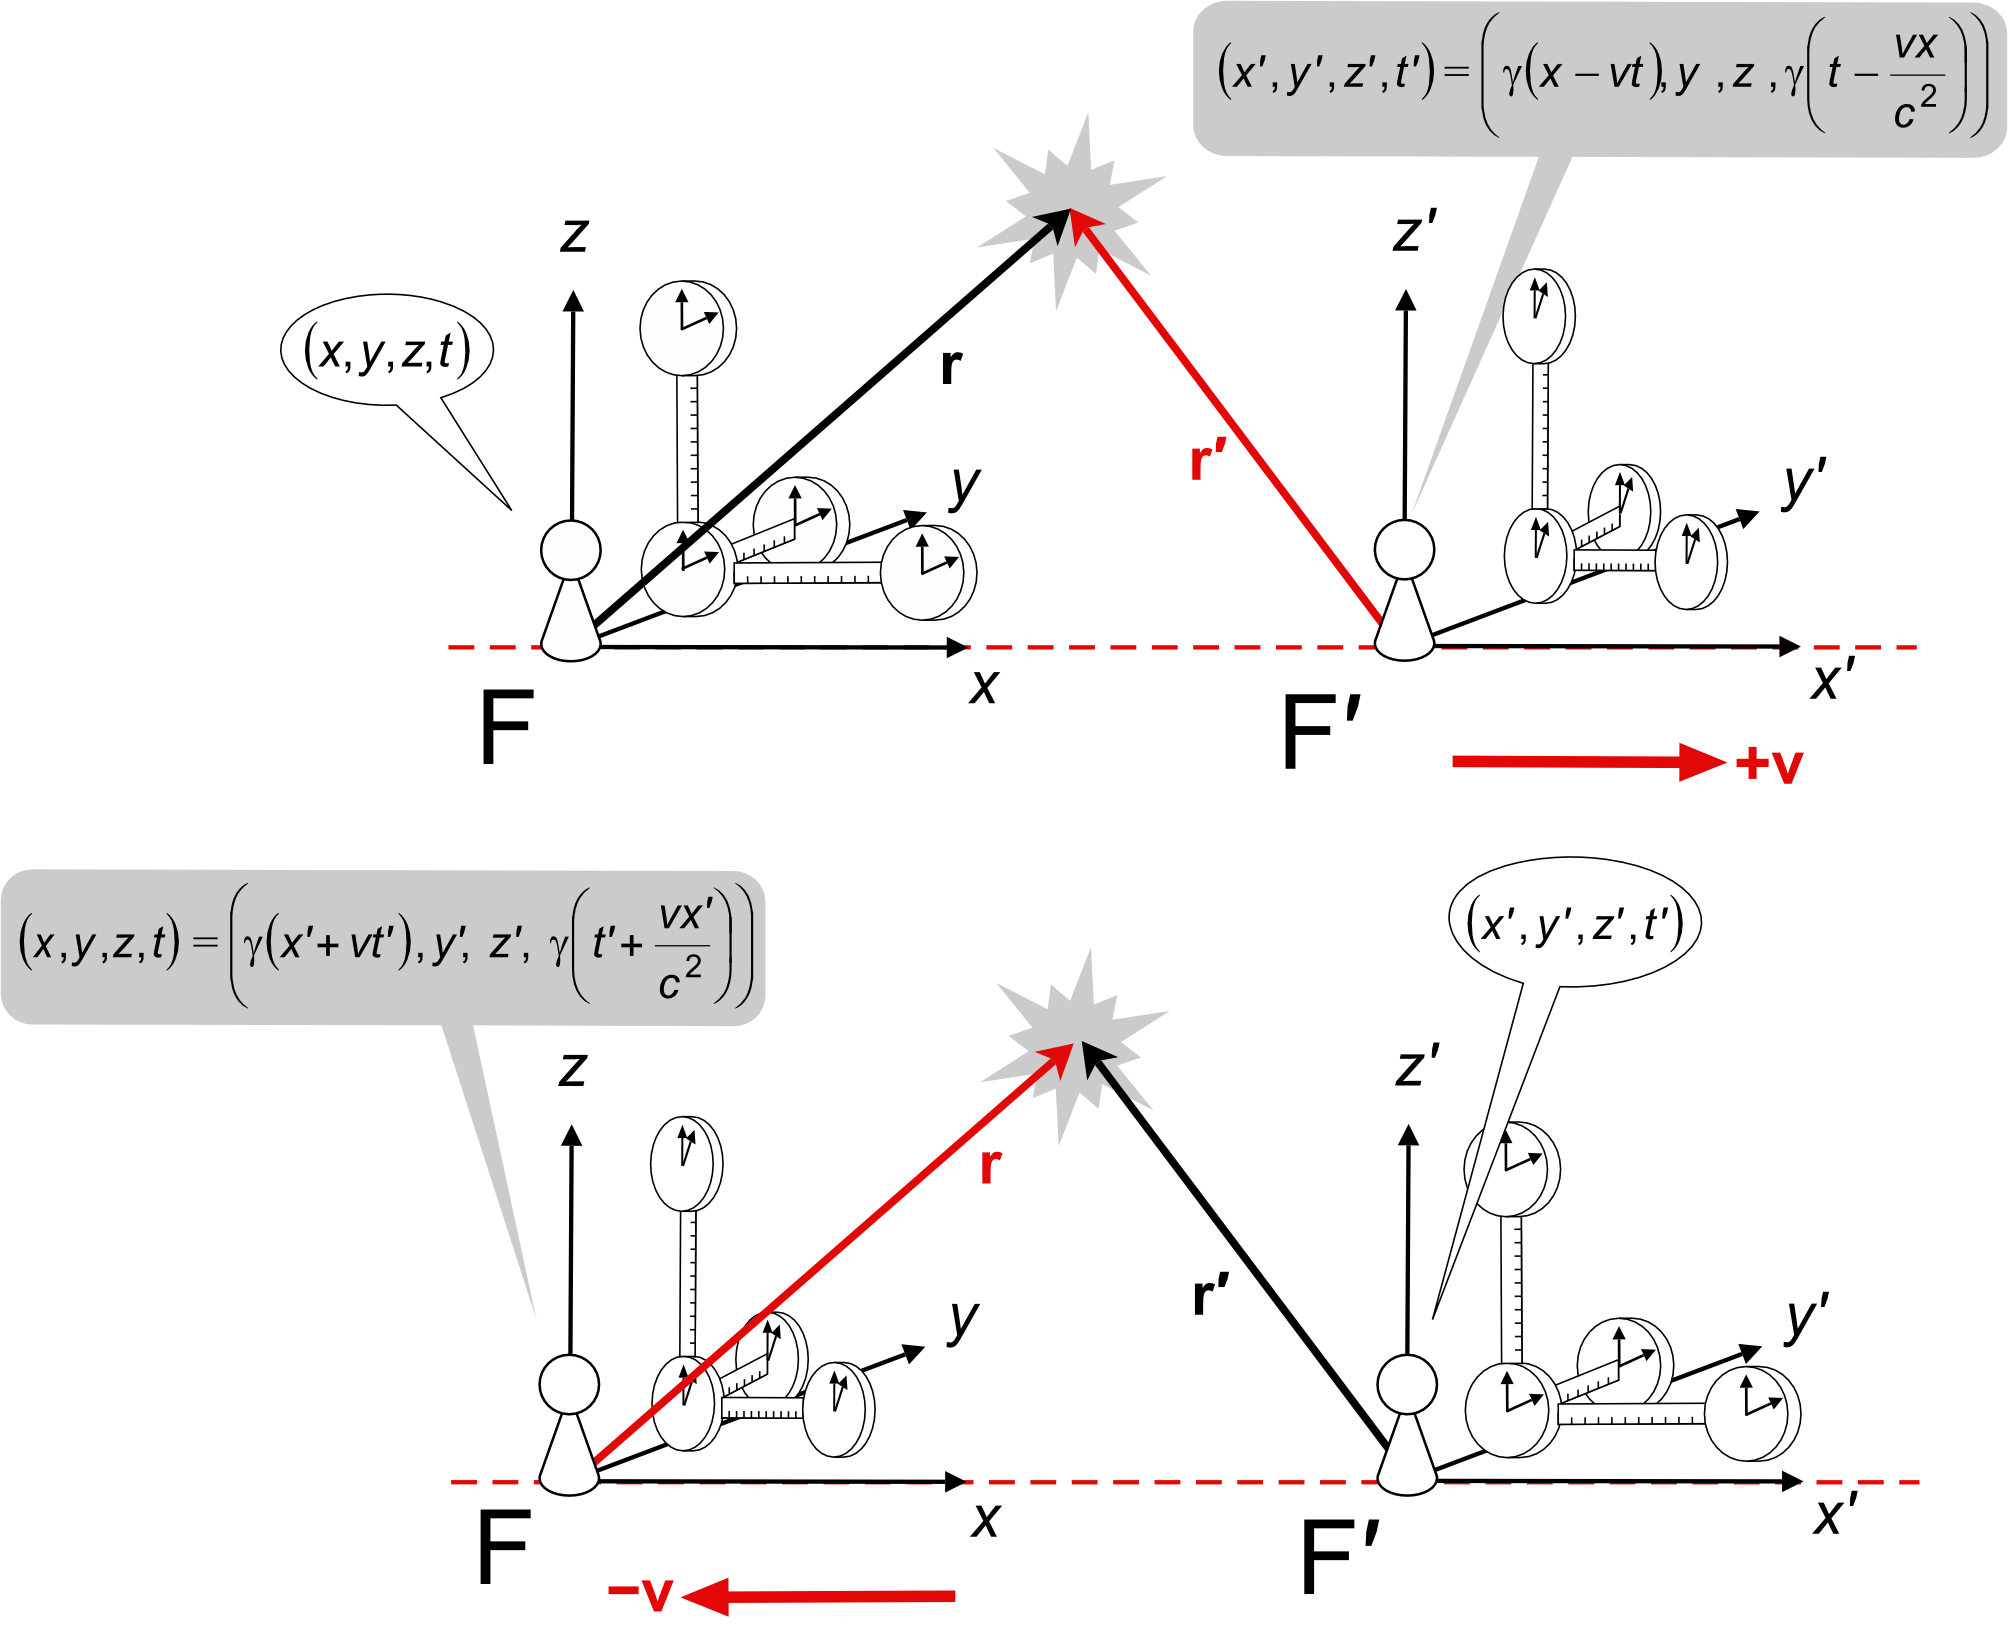
\includegraphics[width = 11cm]{ass1_lorentz_transforms.png}\end{wrapfigure}

Consider two inertial frames of reference \(F\) and \(F'\), with \(F'\) is moving with a velocity \(v\) with respect to \(F\) in the positive \(x\)-direction.

Let coordinates in \(F\) be represented as \((x, y, z, t)\), and the corresponding coordinates in \(F'\) as \((x', y', z', t')\).

\subsection{Spatial Transformations}
Since the transformation must be linear (or otherwise fictitious forces would be introduced), and spatial movement is only in the \(x\) direction, the spatial transformations must be in the form:
\[x' = \gamma x + bt\]
\[y' = y\]
\[z' = z\]

Since an object at rest in frame \(F'\) at \(x' = 0\) moves with velocity \(v\) in frame \(F\), the transformation must satisfy \(x' = 0\) when \(x = v t\). Substituting this into the above equation for \(x'\) gives:
\[0 = \gamma v t + b t\]
\[b = -\gamma v\]
\[\therefore x' = \gamma (x - v t)\]

By the principle of relativity, there is no privileged reference frame, so the inverse transformation must be in the same form, but with the velocity negated:
\[x = \gamma (x' + v t')\]

By the postulate of invariant light speed, the speed of light is the same in all frames of reference, so the transformation must guarantee that \(t = \frac{x}{c}\) when \(t' = \frac{x'}{c}\). Substituting this into the previous two equations gives:
\[x' = \gamma (x - v \frac{x}{c}) = \gamma (1 - \frac{v}{c}) x\]
\[x = \gamma (x' + v \frac{x'}{c}) = \gamma (1 + \frac{v}{c}) x'\]

Multiplying the two equations together and solving for \(\gamma\) (The mathematical discontinuity at \(x x' = 0\) can be ignored due to macroscopic physics being continuous):
\[x x' = \gamma^2 (1 - \frac{v^2}{c^2}) x x'\]
\[\gamma = \frac{1}{\sqrt{1 - \frac{v^2}{c^2}}}\]

Thus the transformations for the spatial coordinates is now complete:
\[x' = \frac{x - v t}{\sqrt{1 - \frac{v^2}{c^2}}}\]
\[y' = y\]
\[z' = z\]

\subsection{Temporal Transformation}
To produce the transformation for time, consider the postulate of invariant light speed again, but with the guarantee rearranged to \(x = c t\) and \(t = \frac{x}{c}\) when \(x' = c t'\). Substituting this into the \(x\) transformation yields:
\[c t' = \gamma (c t - \frac{v x}{c})\]
\[\therefore t' = \gamma (t - \frac{v x}{c^2})\]

Which completes the full set of transformations:
\[x' = \frac{x - v t}{\sqrt{1 - \frac{v^2}{c^2}}}\]
\[y' = y\]
\[z' = z\]
\[t' = \frac{t - \frac{v x}{c^2}}{\sqrt{1 - \frac{v^2}{c^2}}}\]

\section{A burst of \(\pi^+\) mesons (pions) travels down an evacuated beam tube at Fermilab moving at \(\beta = \frac{v}{c} = 0.94\) with respect to the laboratory.}
\subsection{Compute \(\gamma\) for this group of pions.}
\[\gamma = \frac{1}{\sqrt{1 - \beta^2}} \approx 2.9\]

\subsection{The proper (rest frame) mean lifetime of pions is \SI{2.6e-8}{\second}. What mean lifetime is measured in the lab?}
\[\tau = \tau' \gamma \approx \SI{7.6e-8}{\second}\]

\subsection{If the burst contains \(60\,000\) pions, how many remain after the group has travelled \SI{48}{\metre} down the beam tube?}
\[t = \frac{d}{\beta c} \approx \SI{1.7e-7}{\second}\]
\[N = N_0 e^{-\frac{t}{\tau}} \approx 6400\]

\subsection{What would your answer to (2.3) be ignoring time dilation? Comment on this result.}
\[N = N_0 e^{-\frac{t}{\tau'}} \approx 86 \ll 6400\]
If time dilation did not exist, the number of pions remaining would be two order of magnitudes smaller than if it did exist.

\section{Frames \(S\) and \(S'\) are moving relative to each other along the \(x\) and \(x'\) axes. They set their clocks to \(t = t' = 0\) when their origins coincide. In frame \(S\), event 1 occurs at \(\frac{x_1}{c} = \SI{1}{yr}\) and \(t_1 = \SI{1}{yr}\) and event 2 occurs at \(\frac{x_2}{c} = \SI{2.0}{yr}\) and \(t_2 = \SI{0.5}{yr}\). These events occur simultaneously in \(S'\).}
\subsection{Draw a space time diagram showing these events in \(S\).}
\begin{figure}[H]
    \centering
    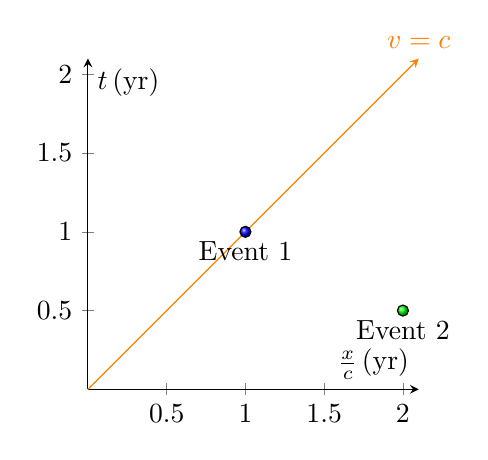
\begin{tikzpicture}
        \begin{axis}[spacetime]
            \addplot[color = orange, domain = 0:2.1, -stealth] {x} node[above, pos = 1] {\(v = c\)};
            \addplot[spacetime event, ball color = blue] coordinates {(1, 1)} node [anchor = north] {Event 1};
            \addplot[spacetime event, ball color = green] coordinates {(2, 0.5)} node [anchor = north] {Event 2};
        \end{axis}
    \end{tikzpicture}
\end{figure}

\subsection{Draw another space time diagram showing these events in \(S'\).}
\begin{figure}[H]
    \centering
    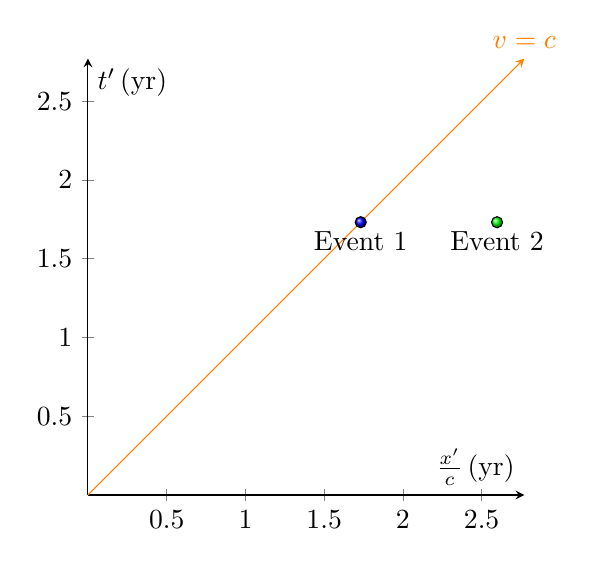
\begin{tikzpicture}
        \begin{axis}[
            spacetime,
            xlabel = \(\frac{x'}{c}\,\mathrm{(yr)}\),
            ylabel = \(t'\,\mathrm{(yr)}\),
            /pgfplots/filter point/.code = {
                \pgfkeysgetvalue{/data point/x}\x
                \pgfkeysgetvalue{/data point/y}\t
    %
                \def\v{-0.5}
    %
                \pgfmathparse{1 / sqrt(1 + \v^2)}
                \let\gamma=\pgfmathresult
    %
                \pgfmathparse{\gamma * (\x - \v * \t)}
                \let\outX=\pgfmathresult
    %
                \pgfmathparse{\gamma * (\t - \v * \x)}
                \let\outT=\pgfmathresult
    %
                \pgfkeyslet{/data point/x}\outX
                \pgfkeyslet{/data point/y}\outT
            }
        ]
            \addplot[color = orange, domain = 0:1.6, -stealth] {x} node[above, pos = 1] {\(v = c\)};
            \addplot[spacetime event, ball color = blue] coordinates {(1, 1)} node [anchor = north] {Event 1};
            \addplot[spacetime event, ball color = green] coordinates {(2, 0.5)} node [anchor = north] {Event 2};
        \end{axis}
    \end{tikzpicture}
\end{figure}

\subsection{Project the \(S'\) axes onto the \(S\) space time diagram and comment on what this shows.}
\begin{figure}[H]
    \centering
    \begin{tikzpicture}
        \begin{axis}[spacetime, xmax = 2.7, ymax = 2.7]
            \addplot[color = orange, domain = 0:2.1, -stealth] {x} node[above, pos = 1] {\(v = c\)};
            \addplot[spacetime event, ball color = blue] coordinates {(1, 1)} node [anchor = north] {Event 1};
            \addplot[spacetime event, ball color = green] coordinates {(2, 0.5)} node [anchor = north] {Event 2};
            \addplot[color = red, domain = -1:2] {1 - (x - 1) / 2};
            \addplot[color = red, domain = 1:2] {1 - 2 * (x - 1)};
            \addplot[color = red, domain = 2:3] {0.5 - 2 * (x - 2)};
        \end{axis}
        \begin{axis}[
            spacetime,
            xlabel style = {xshift = 1cm},
            xlabel = \(\frac{x'}{c}\,\mathrm{(yr)}\),
            x = 2.6cm,
            xmax = 2.7,
            ymax = 2.7,
            anchor = origin,
            rotate around = {atan(-0.5):(current axis.origin)},
            hide y axis
        ]
        \end{axis}
        \begin{axis}[
            spacetime,
            ylabel style = {xshift = 0.2cm},
            ylabel = \(t'\,\mathrm{(yr)}\),
            y = 2.6cm,
            xmax = 2.7,
            ymax = 2.7,
            anchor = origin,
            rotate around = {atan(0.5):(current axis.origin)},
            hide x axis
        ]
        \end{axis}
    \end{tikzpicture}
\end{figure}

Since event 2 occurs before event 1 in frame \(S\) but spatially more distant, this must mean that frame \(S'\) is moving with a negative velocity relative to \(S\), and the diagram shows this, with the primed axes rotated away from the first quadrant.

\subsection{Find the magnitude and direction of the velocity of \(S'\) relative to \(S\).}
\[t'_1 = t'_2 \text{ (Events are simultaneous in \(S'\))}\]
\[\gamma \left(t_1 - \frac{v x_1}{c^2}\right) = \gamma \left(t_2 - \frac{v x_2}{c^2}\right)\]
\[t_1 - \frac{v x_1}{c^2} = t_2 - \frac{v x_2}{c^2}\]
\[v = \frac{t_1 - t_2}{\frac{x_1}{c} - \frac{x_2}{c}} c = -0.5 c\]
\(\therefore S'\) is moving at half the speed of light in the negative \(x\) axis.

\subsection{At what time do both these events occur as measured in \(S'\)?}
\[\gamma = \frac{1}{\sqrt{1 - \frac{v^2}{c^2}}}\]
\[t'_1 = t'_2 = \gamma \left(t_1 - \frac{v x_1}{c^2}\right) \approx \SI{1.7}{yr}\]

\section{Two identical particles of rest mass \(m\) are each moving towards the other with speed \(u\) in frame \(S\). The particles collide inelastically with a spring that locks shut and comes to rest in \(S\), and their initial kinetic energy is transformed into potential energy. In this problem you are going to show that the conservation of momentum in reference frame \(S'\), in which one of the particles is initially at rest, requires that the total rest mass of the system after the collision be \(\frac{2 m}{\sqrt{1 - \frac{u^2}{c^2}}}\).}
\subsection{Show that the speed of the particle not at rest in frame \(S'\) is \(u' = \frac{2 u}{1 + \frac{u^2}{c^2}}\).}
Simply plugging in the two velocities into the relativisitc velocity addition formula yields the answer:
\[u' = \frac{u - (-u)}{1 - \frac{u (-u)}{c^2}} = \frac{2 u}{1 + \frac{u^2}{c^2}}\]

\subsection{Show that \(\sqrt{1 - \frac{u'^2}{c^2}} = \frac{1 - \frac{u^2}{c^2}}{1 + \frac{u^2}{c^2}}\).}
\begin{align*}
    \sqrt{1 - \frac{u'^2}{c^2}} &= \sqrt{1 - \frac{4 u^2}{c^2 (1 + \frac{u^2}{c^2})^2}} \\
    &= \sqrt{1 - \frac{4 u^2 c^2}{(c^2 + u^2)^2}} \\
    &= \sqrt{\frac{(u^2)^2 + 2 u^2 c^2 + (c^2)^2 - 4 c^2 u^2}{(c^2 + u^2)^2}} \\
    &= \sqrt{\frac{(u^2 - c^2)^2}{(c^2 + u^2)^2}} \\
    &= \left|\frac{u^2 - c^2}{c^2 + u^2}\right| = \frac{c^2 - u^2}{c^2 + u^2} \text{ (}\because c > u\text{)} \\
    &= \frac{1 - \frac{u^2}{c^2}}{1 + \frac{u^2}{c^2}}
\end{align*}

\subsection{Show that the initial momentum in frame \(S'\) is \(p' = \frac{2 m u}{1 - \frac{u^2}{c^2}}\).}
Assuming the spring has negligible rest mass, all the initial momentum will be concentrated in the second particle:
\begin{align*}
    p' &= \frac{m u'}{\sqrt{1 - \frac{u'^2}{c^2}}} \\
    &= \frac{2 m u}{1 + \frac{u^2}{c^2}} \cdot \frac{1 + \frac{u^2}{c^2}}{1 - \frac{u^2}{c^2}} \text{ (From (4.1 and 4.2))} \\
    &= \frac{2 m u}{1 - \frac{u^2}{c^2}}
\end{align*}

\subsection{After the collision, the composite particle moves with speed \(u\) in \(S'\) (since it is at rest in \(S\)). Write the total momentum after the collision in terms of the final rest mass \(M\), and show that conservation of momentum implies that \(M = \frac{2 m}{\sqrt{1 - \frac{u^2}{c^2}}}\).}
Once again, assuming the spring has negligible rest mass pre-compression, the momentum will be shared between the two particles, and must be equal to the momentum before collision:
\begin{align*}
    p' &= \frac{M u}{\sqrt{1 - \frac{u^2}{c^2}}} \\
    &= \frac{2 m u}{1 - \frac{u^2}{c^2}} \text{ (From (4.3))} \\
    \therefore \frac{M}{\sqrt{1 - \frac{u^2}{c^2}}} &= \frac{2 m}{1 - \frac{u^2}{c^2}} \\
    M &= \frac{2 m}{\sqrt{1 - \frac{u^2}{c^2}}}
\end{align*}

\subsection{Show that the total energy is conserved in each reference frame.}
\begin{align*}
    E_0 &= \frac{2 m c^2}{\sqrt{1 - \frac{u^2}{c^2}}} \text{ (Total energy of the two particles)} \\
    E_1 &= M c^2 \text{ (Total energy of the composite particle)} \\
    &= \frac{2 m c^2}{\sqrt{1 - \frac{u^2}{c^2}}} \text{ (From (4.4))} \\
    \therefore E_0 &= E_1
\end{align*}
Thus total energy is conserved in the unprimed frame.

\begin{align*}
    E'_0 &= m c^2 + \frac{m c^2}{\sqrt{1 - \frac{u'^2}{c^2}}} \text{ (Total energy of the two particles)} \\
    &= m c^2 \left(1 + \frac{1 + \frac{u^2}{c^2}}{1 - \frac{u^2}{c^2}}\right) \text{ (From (4.2))} \\
    &= \frac{2 m c^2}{1 - \frac{u^2}{c^2}} \\
    E'_1 &= \frac{M c^2}{\sqrt{1 - \frac{u^2}{c^2}}} \text{ (Total energy of the composite particle)} \\
    &= \frac{2 m c^2}{1 - \frac{u^2}{c^2}} \text{ (From (4.4))} \\
    \therefore E'_0 &= E'_1
\end{align*}
Thus total energy is conserved in the primed frame.

\section{A positive charge of \SI{7.00}{\pico\coulomb} is spread uniformly along a thin non-conducting rod of length \(L = \SI{2.00}{\centi\metre}\). What are the magnitude and direction (relative to the positive direction of the \(x\) axis) of the electric field produced at point \(P\), at a distance \(R = \SI{8.00}{\centi\metre}\) from the rod along its perpendicular bisector?}
No thickness is specified for the rod, so assuming it is small enough relative to the distance away such that an infinitely thin line is a good approximation.

Since the charges are spread over a finite length straight line, we can use the superposition principle and integrate Coulomb's law over the line. The electric field will also be radially symmetric, so we only need to consider the two dimensions: along the axis of the line and radially away from the line.
\begin{align*}
    \mathbf{E} &= \frac{1}{4 \pi \varepsilon_0} \int_{\mathbf{r'}} \lambda(\mathbf{r'}) \frac{\mathbf{r} - \mathbf{r'}}{|\mathbf{r} - \mathbf{r'}|^3} \, \mathrm{d}\mathbf{r'} \\
    \lambda &= \frac{q}{L} \\
    \mathbf{r} &= (0, R) \\
    \mathbf{r'} &= (s, 0) \text{ where } s \in \left[-\frac{L}{2}, \frac{L}{2}\right] \\
    \therefore \mathbf{E} &= \frac{q}{4 \pi L \varepsilon_0} \begin{pmatrix}
        \int_{-\frac{L}{2}}^{\frac{L}{2}} \frac{-s}{(R^2 + s^2)^{\frac32}} \, \mathrm{d}s \\
        \int_{-\frac{L}{2}}^{\frac{L}{2}} \frac{R}{(R^2 + s^2)^{\frac32}} \, \mathrm{d}s
    \end{pmatrix} \\
    &= \frac{q}{4 \pi L \varepsilon_0} \begin{pmatrix}
        0 \\
        \frac{2 L}{R \sqrt{L^2 + 4 R^2}}
    \end{pmatrix} \\
    &= \begin{pmatrix}
        0 \\
        \frac{q}{2 \pi \varepsilon_0 R \sqrt{L^2 + 4 R^2}}
    \end{pmatrix} \\
    &\approx \begin{pmatrix}
        0 \\
        6.14
    \end{pmatrix}\SI{}{\newton\per\coulomb}
\end{align*}
\(\therefore \mathbf{E}\) is approximately \SI{6.14}{\newton\per\coulomb} pointing away from the rod.

\section{The volume charge density of a solid non-conducting sphere of radius \(R = 10.0\,\mathrm{cm}\) varies with the radial distance \(r\) as given by \(\rho = (20.0\,\mathrm{pC \cdot m^{-3}})\frac{r^2}{R^2}\).}
\subsection{What is the sphere's total charge?}
Since the volume density only depends on radial distance, it is spherically symmetric. This means we can calculate the total charge by integrating sphere surfaces of charges over the radius.
\begin{align*}
    \text{let } k &= 20.0\,\mathrm{pC \cdot m^{-3}} \\
    q &= \int_0^R \rho(r) 4 \pi r^2 \, \mathrm{d}r = \frac{4 k \pi}{R^2} \int_0^R r^4 \, \mathrm{d}r \\
    &= \frac{4 k \pi R^3}{5} \\
    &\approx 5.03 \times 10^{-14}\,\mathrm{C}
\end{align*}

\subsection{What is the field magnitude, \(E\), at \(r = 0\)?}
Due to the spherical symmetry, \(E = 0\,\mathrm{N \cdot C^{-1}}\)

\subsection{What is the field magnitude, \(E\), at \(r = \frac{R}{2.00}\)?}
We can consider the field to be the superposition of the inner solid sphere with radius \(r\) and the outer hollow sphere with inner radius \(r\) and outer radius \(R\). There exists no electric field inside a spherically symmetrically charged hollow sphere, so we can ignore it and only consider the inner solid sphere.

Applying Gauss' law at radius \(r\) with a spherical Gaussian surface will allow us to solve for \(E\), as follows:
\begin{align*}
    \frac{Q}{\varepsilon_0} &= \oiint_S \mathbf{E} \cdot \mathrm{d}\mathbf{A} = 4 \pi r^2 E \\
    \therefore E &= \frac{Q}{4 \pi \varepsilon_0 r^2} \\
    Q &= \frac{4 k \pi}{R^2} \int_0^r r^4 \, \mathrm{d}r = \frac{4 k \pi r^5}{5 R^2} \text{ (Similar to (6.1))} \\
    \therefore E &= \frac{k r^3}{5 R^2 \varepsilon_0} \\
    \therefore E\bigg|_{r=\frac{R}{2.00}} &\approx 5.65 \times 10^{-3}\,\mathrm{N \cdot C^{-1}}
\end{align*}

\subsection{What is the field magnitude, \(E\), at \(r = R\)?}
Same process as above, but the ignored outer sphere actually does not exist in this case.
\[E\bigg|_{r=R\,\mathrm{cm}} \approx 4.52 \times 10^{-2}\,\mathrm{N \cdot C^{-1}}\]

\subsection{Carefully graph \(E\) versus \(r\) showing as many details as possible.}
Outside of the sphere, we take a spherical Gaussian surface again, but with \(Q = q\big|_{R = R}\), to obtain the formula \(E = \frac{k R^3}{5 r^2 \varepsilon_0}\). The electric field magnitude both inside and outside of the sphere is graphed below:

\begin{figure}[h]
    \centering
    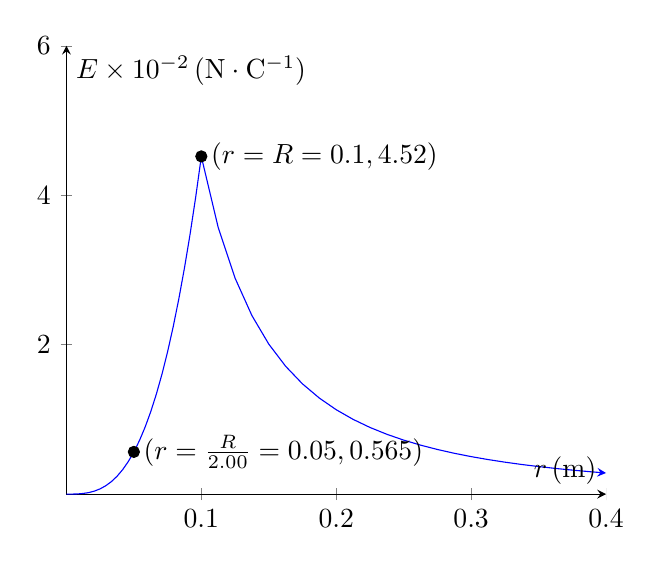
\begin{tikzpicture}
        \begin{axis}[
            axis lines = middle,
            clip = false,
            xlabel = \(r\,\mathrm{(m)}\),
            ylabel = \(E\times 10^{-2}\,\mathrm{(N \cdot C^{-1})}\),
            ymax = 6
        ]
            \def\k{20e-12}
            \def\R{0.1}
            \def\epsilon{8.854e-12}
            \addplot[color = blue, domain = 0:0.1] {100 * \k * x^3 / (5 * \R^2 * \epsilon)};
            \addplot[color = blue, domain = 0.1:0.4, -stealth] {100 * \k * \R^3 / (5 * \epsilon * x^2)};
            \addplot[only marks] coordinates {(0.05, 0.565)} node [anchor = west] {\((r = \frac{R}{2.00} = 0.05, 0.565)\)};
            \addplot[only marks] coordinates {(0.1, 4.52)} node [anchor = west] {\((r = R = 0.1, 4.52)\)};
        \end{axis}
    \end{tikzpicture}
\end{figure}

\end{document}
